\begin{figure}[h!]
\centering
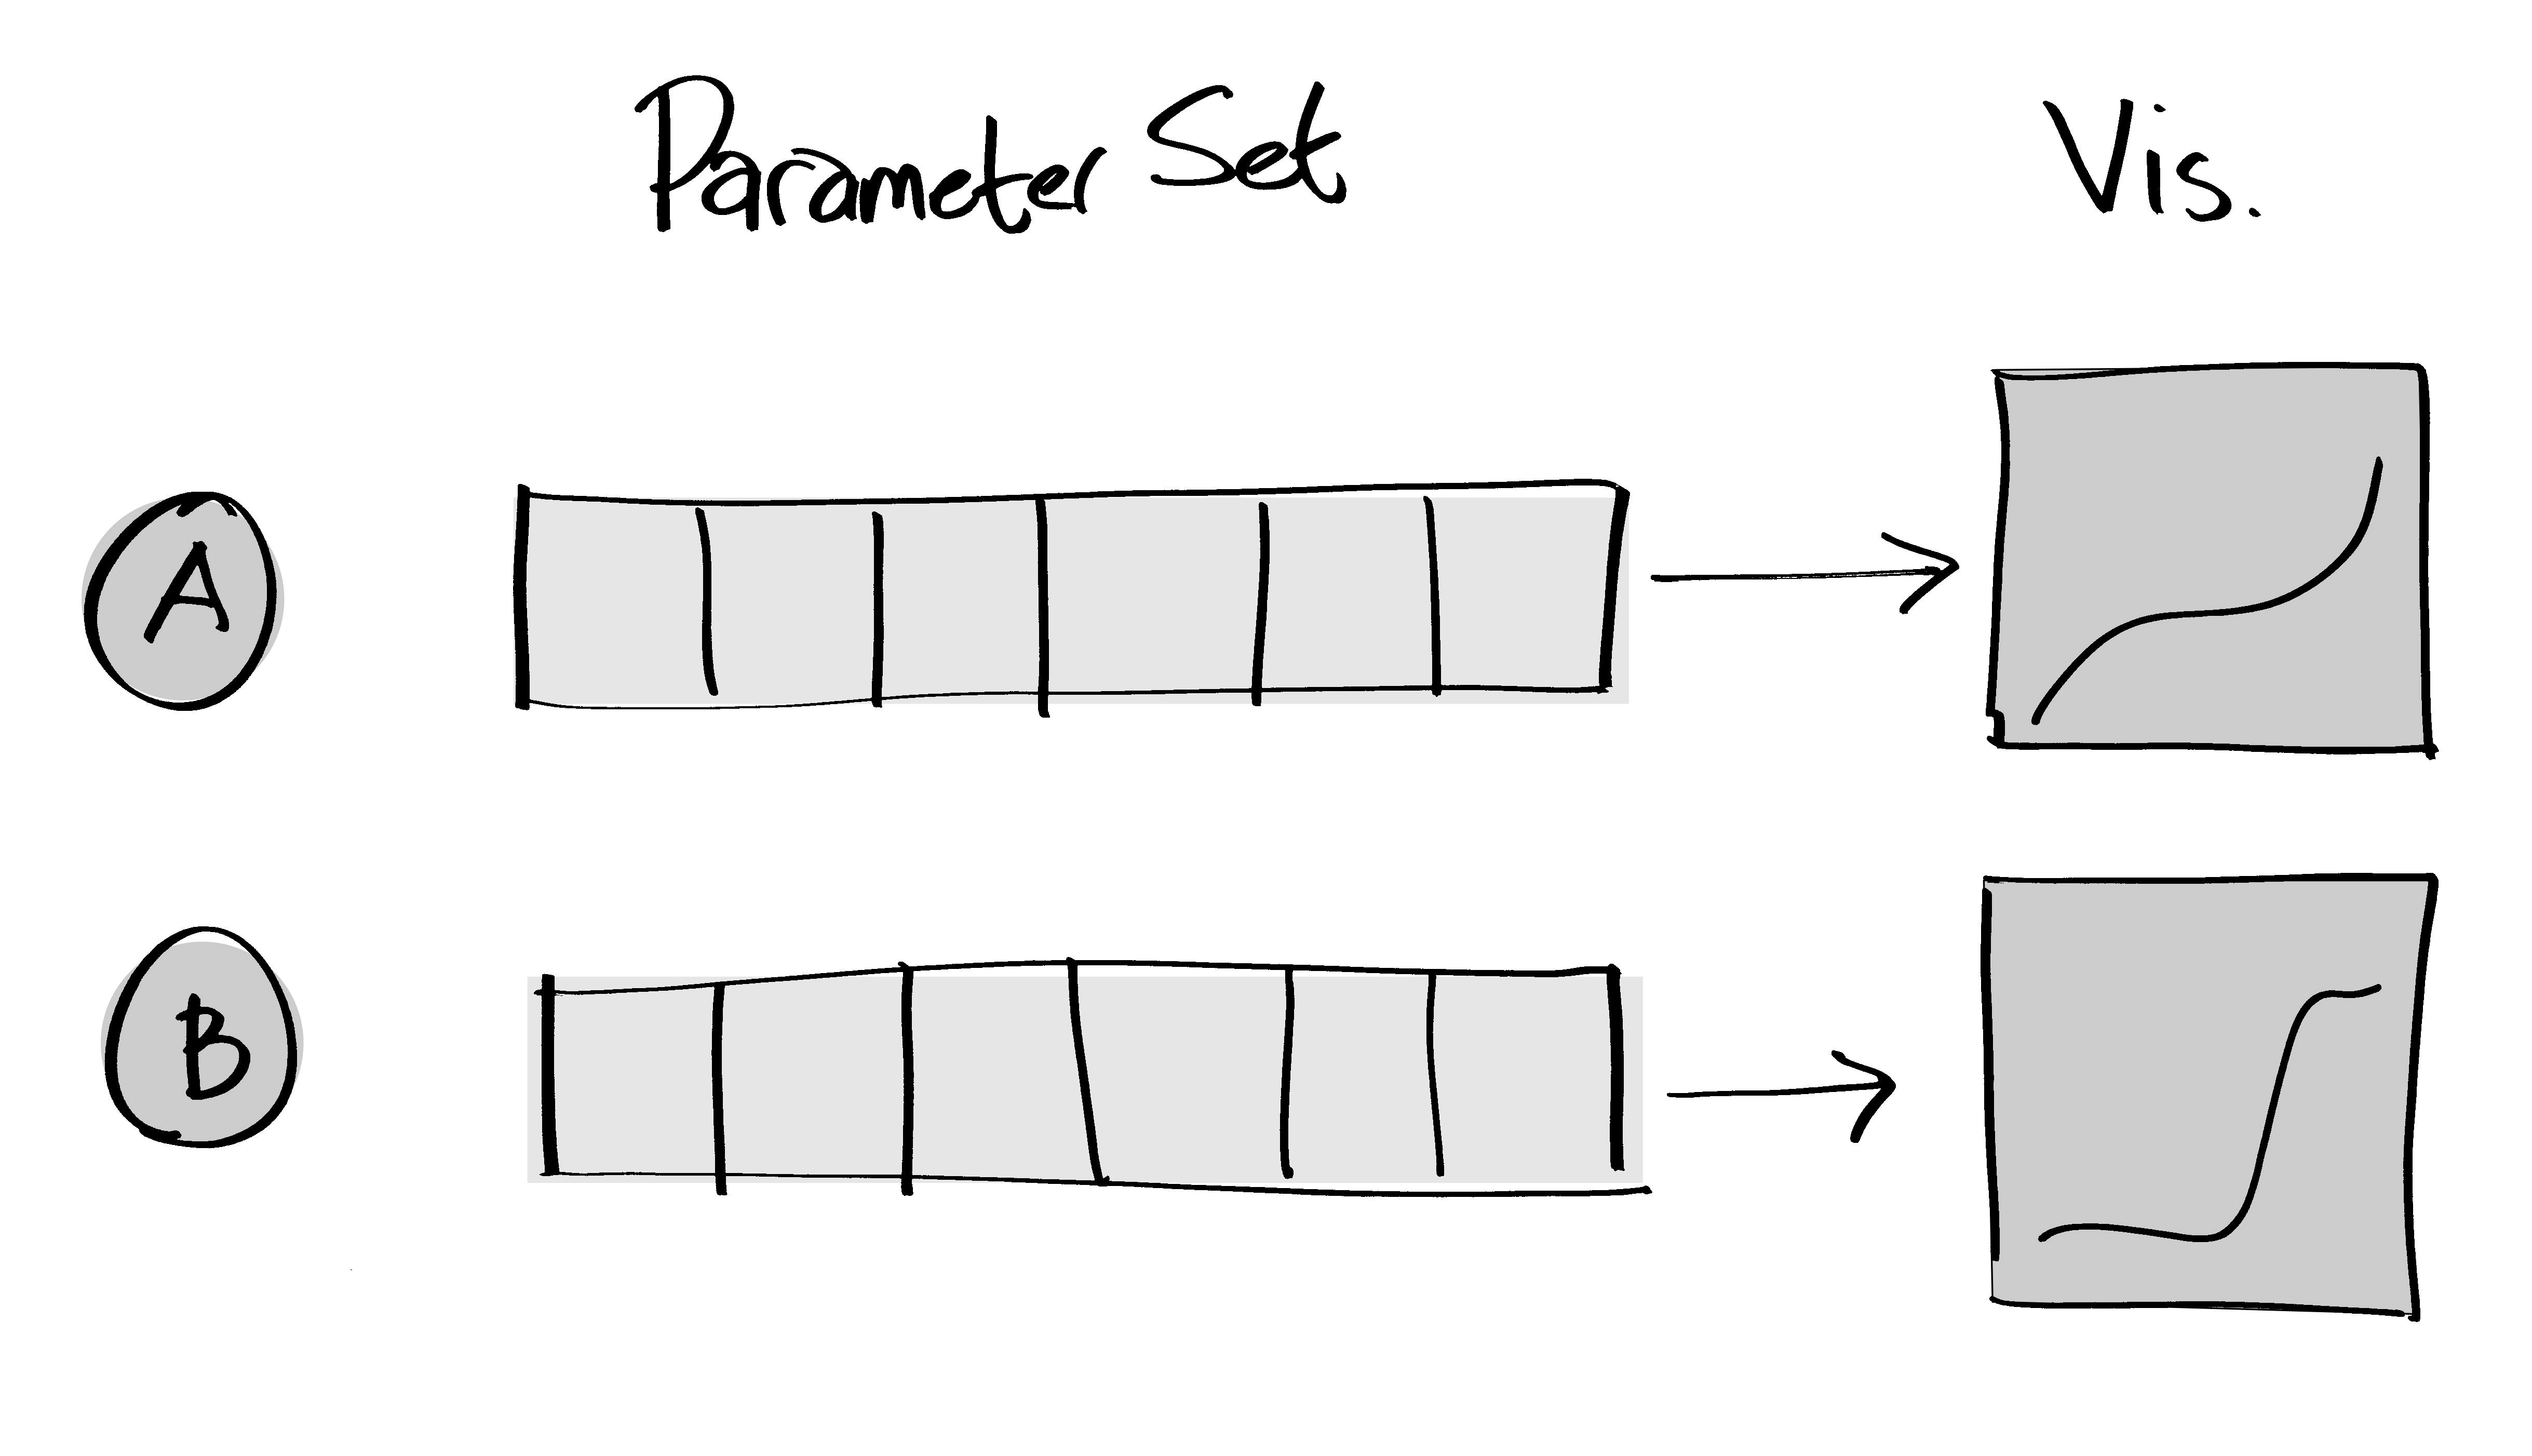
\includegraphics[width=0.8\textwidth]{img/parameter_set_diagram_filled}
\caption{
    Diagram showing a typical set of data that a scientist has for an experiment or simulations. Some set of parameters (A or B) has been used to create a visualization - a graph, an image captured from a sensor, or other data. These parameter sets can include, for example, settings on an experimental machine, inputs to a simulation, or measurements taken by a sensor. Each one of the parameter sets thus defines a unique result. Taken together, a set of these parameter sets constitutes a database of results, and a scientist often tracks this database in a spreadsheet. These parameter set/image pairings form the basis for the simplest Spec D database.
}
\label{fig:parametersets}
\end{figure}
